\documentclass[a4paper,11pt]{article}

\usepackage{amssymb}
\usepackage{amstext}
\usepackage{amsmath}
\usepackage{amsthm}
\usepackage{booktabs}
\usepackage{graphicx}
\usepackage{float}
\usepackage{url}
\usepackage{proof}
\usepackage{hyperref}
\usepackage{multicol}

\usepackage{bussproofs}

\usepackage{algorithm}
\usepackage{arevmath}     % For math symbols
\usepackage[noend]{algpseudocode}

\theoremstyle{definition}
\newtheorem{definition}{Definition}[section]

\usepackage{xcolor}
\newcommand{\bluenote}[1]{\color{blue}{ \em #1 }\color{black}}

\usepackage{geometry}
 \geometry{
 a4paper, %letterpaper,
 total={17cm,22.8cm},
 margin=24mm,
 top=22.4mm,
 bottom=25.4mm
 }
 
% Times new roman
\usepackage{mathptmx}

\usepackage[T1]{fontenc}

\usepackage{caption}
\usepackage{subcaption}

\thispagestyle{empty} 

\setlength{\parindent}{0pt}

% For comment boxes.
\usepackage[colorinlistoftodos,prependcaption,textsize=tiny]{todonotes}
\newcommand{\giselle}[1]{\todo[linecolor=red,backgroundcolor=red!25,bordercolor=red]{G: #1}}
\newcommand{\samar}[1]{\todo[linecolor=blue,backgroundcolor=blue!25,bordercolor=red]{S: #1}}

\author{%
%  \fontsize{10}{12}\selectfont
  \begin{minipage}[t]{0.47\textwidth}
    \centering
    Samar Rahmouni \\ srahmoun@andrew.cmu.edu
  \end{minipage}
  \and
  %
  \begin{minipage}[t]{0.45\textwidth}
    \centering
    Advisor: Prof. Giselle Reis \\ giselle@cmu.edu
  \end{minipage}%
  \vspace*{2ex}
}


\date{}

\title{{\Large\sc Senior Thesis 2021-22\\[2ex]}{\LARGE\bf Domained
Informed Oracle (DIO)\\ in Reinforcement Learning}\\}


\begin{document}

\maketitle 

\begin{abstract} 

  %% The story

  %% There is this great new method!
  Reinforcement learning (RL) is a powerful AI method that does not
  require pre-gathered data but relies on a trial-and-error process
  for the agent to learn. 
  %
  This is made possible through a reward function that associates
  current state configurations to a numerical value. 
  %
  The agent's goal is then to maximize its cumulative reward over its
  lifetime. 
  % 
  %% Oh, but there are some issues...
  Unfortunately, there is no systematic method to design a reward
  function.
  %
  This needs to be done on a case by case basis, and might be hard
  depending on how the states are represented.
  %
  States are typically represented as vector of values in RL, and
  translating properties and rules from a domain into this
  representation can be complicated depending on how many values are
  used, what they represent, whether they are normalized or not, etc.


%  \medskip

  % This is needed to connect the ideas from the previous paragraph
  % and the next.

%%   %% No problem, we can solve them!
%%   These challenges can be alleviated for a given domain by fine
%%   tuning the reward function with domain specific information. 
%%   %
%%   For example, if the agent is a self-driving car, the reward function
%%   can include the physics equations to predict, with some degree of
%%   certainty, the car's trajectory for the next few seconds.
%%   %
%%   By looking into the future, the reward function can penalize bad
%%   behavior before it reaches a catastrophic state (\emph{e.g.}, a
%%   crash).
%%   %
%%   A better reward function prunes the (often infinite) search space
%%   faster, allowing the agent to explore (breadth) new states instead
%%   of exploiting (depth) dead ends.
%%   %
%%   %% Oh, but only on a case by case basis...
%%   However, tuning the reward might be hard depending on the domain and
%%   how states are represented.
%%   %
%%   States are typically represented as vector of values in RL, and
%%   translating properties and rules from a domain into this
%%   representation can be complicated depending on how many values are
%%   used, what they represent, whether they are normalized or not, etc.

%  \medskip

  %% We can fix that!
  We propose a \emph{Domain Informed Oracle (DIO)} as a solution for
  systematically incorporating domain specific knowledge into RL
  reward functions.
  %
  DIO is a collection of domain specific rules written in a
  declarative language, such as Prolog.
  %
  It does not rely on the RL representation of states, allowing the
  programmer to focus on the domain specific knowledge using an
  expressive and intuitive language, where they can define states and
  rules in the most convenient way.
  %
  DIO provides an informed decision to the reward function, thus
  allowing it to dynamically adapt the rewards. 
  %
  %DIO is incorporated into a RL architecture and is defined by its
  %behavior in relation to the input given by the reward function. 
  
  Our implementation is tested on a Traffic Simulator scenario and
  compared to a basic uninformed RL algorithm. 
  %
  The comparison is based on performance which we define by three
  metrics: time to train, optimality of the learned policy and
  finally, number of errors states reached. 
  
\end{abstract}



\section{Introduction}

Implementing a robust adaptive controller that is effective in terms
of precision, time, and quality of decision
when facing dynamic and uncertain scenarios, has always been a central
challenge in AI and robotics. Precisely, as we want our autonomous agents to be deployed 
in the real world, we want to ensure that they are able to adapt to unforeseen scenarios, as well as 
keep their efficiency. This efficiency is measured in terms of their optimality and time taken to produce a decision. 
%
As autonomous cars are deployed, IoT is popularized, and human-robot interactions become more complex, we
are more and more confronted with the need for robotic agents that can effectively and continually adapt
to their surroundings, not only in simulation, but also in practice, when deployed as a cyber-physical system. 
Since we are unable to provide a repertoire of all possible scenarios and actions,
our agents need to be able to autonomously predict and adapt to new
changes. Reinforcement Learning (RL) is an approach that
supports dynamically adapting to new input. It is also the solution that AlphaGo, Deepmind AlphaStar, and OpenAI Five have
adopted \cite{li2019reinforcement}, respectively for Go, StarCraft II and Dota 2 and found success in. 

\medskip

Reinforcement Learning is a powerful tool as it does not require
pre-gathered data as most Machine Learning (ML) techniques do. 
%
The general idea of RL is a trial-and-error process guided by a
\textit{domain dependent} reward function.
%
For example, if the agent is a self-driving car, the reward function
can greatly penalize states when it crashes.
%
However, this means that the car is bound to crash to learn not to
crash again.
%
A better reward function can include the physics equations to predict,
with some degree of certainty, the car's trajectory for the next few
seconds.
%
By looking into the future, the reward function can penalize bad
behavior before it reaches a catastrophic state (a crash).
%
A better reward function prunes the (often infinite) search space
faster, allowing the agent to explore (breadth) new states instead of
exploiting (depth) dead ends.
%
%For example, say we want to teach an autonomous car to stop at a STOP
%sign. We will punish it via a negative reward when it does not,
%otherwise, we will reward it. Thus, through multiple iterations, and
%with the goal to maximize its rewards, a reinforcement learning
%trained agent will learn to stop at a STOP sign. 

\medskip

The task of choosing a reward function that ensures optimality is thus
crucial. 
%
In this work, we propose a Domain Informed Oracle (DIO) written in a
declarative language to inform a reinforcement learning algorithm. 
%
Our method provides a systematic way to encode domain specific rules
into a reward function for RL that does not rely on the state
representation within the RL algorithm.
%
We argue that such a combination will ensure a faster and more
efficient RL trained agent in terms of optimality. 
%
The proposed combination is tested on a traffic simulation and the
results are compared with a RL implementation that makes use of
standard practices to design a reward function. 


%% Reinforcement Learning from basics to challenges to significance
\section{Reinforcement Learning} 

Reinforcement Learning is a method of learning that maps situations to
actions in order to maximize its rewards
\cite{sutton2018reinforcement}. Rewards are numerical values associated to a state and action. Precisely, one defines a reward function 
$R : (S \times A) \rightarrow \mathbb{R}$ where $S$ defines the state space and $A$ the action space. Note that a state refers to the current configuration
of the environment and the action refers to the action chosen by the RL agent. By defining this reward function and the scenario of the problem the agent is trying to solve, 
reinforcement learning has the advantage of not requiring a prior dataset. Indeed, the agent is not told what to do, but rather 
learns from the effect of its actions on the environment. 
% Consider Figure~\ref{fig:rl}. [GR] You are explaining the figure in
% the next paragraph, so this sentence is not needed.

\begin{figure}[H]
  \centering
  
\includegraphics[scale=0.6]{figures/rlroutine.png}
  \caption{Reinforcement Learning Routine}
  \label{fig:rl}
\end{figure}


The diagram in Figure~\ref{fig:rl} is a high-level description of how
an agent using reinforcement learning can be trained.  
%
The lower box represents the \emph{environment} as seen by the agent
according to its sensors.
%
The current state of the environment is represented as a \emph{state
vector}.
%
At each iteration, the agent will receive the state vector as input,
and needs to choose an \emph{action} to take.
%
Once the action is taken, the environment is updated to the next state
and the agent receives a \emph{reward} as feedback.
%
This reward is a domain dependent function that represents how
``good'' the state is.
%
The agent's goal is to increase its reward by taking actions that
reach better states each time.

\medskip 

The reward function is a crucial aspect of the RL algorithm. For instance, consider a game of chess 
where the agent is punished when it loses and rewarded if it wins. The agent is bound to learn how to 
maximize its winnings but it will need to exhaust multiple possible combinations to learn. In this case, 
the training time is not optimal. A better approach would be to also reward it for making a good opening, for instance. 
Another example would be only considering negative rewards. Say we want our agent to escape a maze, and we punish it at every timestep for not escaping. 
If there is a fatality state (\emph{e.g.}, a fire or a black whole), the agent will learn to move towards the fatality state as to cut its negative rewards as soon as possible. 
In conclusion, a good reward function is the first step of optimal learning. By choosing the right reward function, 
we can ensure a faster and more efficient training, possibly with fewer errors. 

\subsection{Challenges in Reinforcement Learning}
\label{sec:challenges}

Reward shaping (1), the exploration-exploitation dilemma (2) and
meta-learning (3) are main challenges
that make it harder for RL to be adopted as a solution to more real-world problems. 

\medskip 

\emph{Reward shaping}~\cite{laud2011} refers to the lack of systematic methods to design a reward
  function that ensures fast and efficient learning. This generation of an appropriate 
reward function for a given problem is still an open challenge~\cite{kober2013}.
Ideally, rewards would be given by the real-world, i.e. \textit{native rewards}. For instance, recent work investigates dynamically generating a reward 
using a user verbal feedback to the autonomous agent~\cite{gonzalez2010}. However, most RL agents 
can only stay in simulation due to the lack of safety guarantees. This is because of the trial-and-error nature of the RL training. 
Thus, there exists a need for \textit{shaping rewards} instead. There are reasonable criteria on how this should be done, those are \emph{standard practices}. For instance, 
rewards that can be continuously harvested speed up convergence
compared to rewards that can only be harvested at ``the end''
(\emph{i.e.} the chess example). Similarly, one should avoid only 
negative rewards as that results in unwanted behavior. Furthermore, if dealing with a continuous state space, it helps to have a polynomial differential function as the reward function 
as it is shown to help the agent learn faster. Finally, one can normalize rewards at the end as to not end up with too many discrepancies. 
However, there still exists a lack of a systematic method to design a
reward function, and this needs to be done on a case by case basis.
%
Moreover,\giselle{I think this is one of the main points you should
make about DIO, but it is mentioned here in an \emph{en passant}
style, which diminishes its importance.} the abstract representation of states and actions can make
it difficult to map domain specific rules and judgments to the reward
function. A consequence of finding a systematic method to shaping
rewards handles (2), namely, the exploitation vs. exploration
dilemma.\giselle{I added the ``namely'' part because at this point the
definition of (2) was too long ago.}

\medskip

The \emph{exploration vs. exploitation dilemma} is the question of whether to always exploit what the
agent knows or explore in the hope that an unexplored state might
result in better rewards. This dilemma of \emph{exploration} vs. \emph{exploitation} is a central issue of RL. Consider this problem. An agent is at an intersection. It has the choice of going either right or left. 
It does not yet know the outcome of either. It chooses right at a given point and receives a reward $r=1$. The question is "When faced with the same decision, should it keep going right?" There are two issues to consider. 
First, it does not know the outcome of going left. It could be that there is a better reward waiting for it on the left lane. Second, when dealing with a stochastic environment, it might be that $r$ was a one-time occurence. 
It would be equivalent to someone buying a lottery ticket, and winning
\$1M on their first try, and thus, spending all that they won in trying to make it happen again. This problem showcases the importance of exploration; an agent 
needs to see where other paths might lead to, but also exploitation; if it keeps exploring forever it will never accumulate rewards. This is especially evident when the possible states cannot be exhausted. Several techniques have been proposed 
to balance between exploration and exploitation \cite{Kaelbling1996ReinforcementLA}. A notable one is the \emph{epsilon-greedy} technique. The idea is to set some probability $\epsilon$ by which the agent decides to explore. This probability can be adapted 
to decrease as more \emph{episodes} are completed. However, by ensuring (1), an informed reward function is able to sufficiently 
deter the exploration of undesirable states while encourage the exploitation of desirable ones, continuously adapting to 
acquired knowledge and resolving the conflict when necessary. More interestingly, a solution to (2) impacts (3). 


\medskip

\emph{Meta-learning} is the problem of deploying an agent trained in a simulation to
the real-world, or possibly another simulation, where it encounters
state configurations it did not during its training. The goal is to
be able to efficiently adapt to those configurations. The problem of meta-learning in RL stems from the uncertainties of the world. 
Consider the result of training: a function $\pi$ that map states to
actions $\pi : S \rightarrow A$. The learned policy is the one that maximizes the cumulative rewards.
This training is most often done in simulation, given the lack of safety guarantees of RL. 
However, several problems come into place when considering the deployment of the trained agent. Considering that an agent has done well in 
a designated simulation does not imply that it will do as well in the real-world. Overall, it must be that certain uncertainties will not be expected, thus there can be no expectation on how the agent will behave 
when out of simulation. Meta-learning in reinforcement learning is the problem of learning-to-learn, which is about efficiently
adapting a learned policy to conditions and tasks that were not encountered in the past. In RL, meta-learning
involves adapting the learning parameters, balancing exploration and exploitation to direct the
agent interaction \cite{gupta_meta-reinforcement_2018,schweighofer_meta-learning_2003}. Meta-learning is a central problem in AI, since an agent that can solve more
and more problems it has not seen before, approaches the ideal of a general-purpose AI. However, as noted previously, a solution to (2) implies 
a continuous adaptation to knowledge. Since the conflict of exploration and exploitation is resolved, the agent adapts accordingly to tasks it encountered in the past (exploiting), but also 
tasks it encounters for the first time (exploring). Thus, from (2) one
can have a significant impact on (3).


%% Overview of the proposed solution as symbolic reasoning for RL
%% Should separate this to include in related work or change title to make it clearer?
\section{Symbolic Reasoning for Reinforcement Learning} 
\label{symrl}

To tackle the challenges from Section~\ref{sec:challenges}, we are
inspired by the current Neurosymbolic AI trends, which explore
combinations of deep learning (DL) and symbolic reasoning.
%
The work has been a response to criticism of DL on its lack of formal
semantics and intuitive explanation, and the lack of expert knowledge
towards guiding machine learning models.
%
A key question the field targets is identifying the necessary and
sufficient building blocks of AI~\cite{garcez2020neurosymbolic},
namely, how can we provide the semantics of knowledge, and work
towards meta-learning? 
%
Current Neurosymbolic AI trends are concerned with knowledge representation and reasoning, namely, they investigate computational-logic systems 
and representation to precede learning in order to provide some form of incremental update, e.g. a meta-network to group two sub-neural networks. \cite{Besold2017NeuralSymbolicLA}
This leads to neurosymbolic AI finding various applications including vision-based tasks such as semantic labeling \cite{vinyals2015, karpathy2015}, 
vision analogy-making \cite{Reed2015DeepVA}, or learning communication protocols \cite{Foerster2016LearningTC}. Those results inspire us to use those techniques for reinforcement learning, as to tackle its challenges.

\medskip
Rewards are domain dependent and thus, given domain specific rules, a \emph{domain informed} module can guide a RL agent towards better decisions. This can be done by 
adapting the reward function. For instance, we consider defining which states are desirable, which are to be avoided and which are fatal. Given rules and judgments, a logic programming module 
is able to search the space and send feedback to the reinforcement learning agent. The goal is a systematic method to design a reward function which can ensure faster and more efficient 
training. This knowledge can furthermore be incorporated into resolving the exploration vs. exploitation dilemma. For instance, if a domain informed module 
can infer that only one of the possible next states is desirable, then exploration in that specific case is suboptimal.  
We will call the proposed module a \emph{Domain Informed Oracle (DIO)}. 

\begin{figure}[H]
  \centering
  
\includegraphics[scale=0.5]{figures/overview.png}
  \caption{Overview of the proposed solution}
  \label{fig:overview}
\end{figure}

The diagram in Figure~\ref{fig:overview} is a high-level description of our proposed solution. 
%
The box on the left represents a basic reinforcement learning algorithm that depends on the scenario of the given problem and 
the common standard practices discussed previously to design a reward function. 
%
The box on the right represents our proposed domain knowledge to inform the reinforcement learning algorithm. 
Precisely, the domain informed oracle is given the scenario and can thus start a feedback loop between itself and 
the informed RL module to update the rewards. 
%
Finally, those two implementations will be compared based on their performance. In the following, we define performance 
given three metrics: (1) time to train (2) optimality of the learned policy and (3) number of errors through training. 
Consider 'errors' as suboptimal decisions that were made by the agent while in the process of training. For example, exploring a (state, action) pair 
that has previously given a negative reward is suboptimal. 


%% Domain Informed Oracle : Architecture, specifications and modules interactions
\section{Domain Informed Oracle} 
\subsection{Architecture}
In this section, we lay the foundations of the architecture that combines the Domain Informed Oracle with 
reinforcement learning. Note that in our proposed architecture, we suppose Proximal Policy Optimization, a specific method to compute the policy in RL that is explained in more details in \ref{sec:rldetails}. 
It does not mean that our solution is specific to it, rather it can be generalized to any algorithm choice.

\medskip 

\begin{figure}[H]
  \centering
  \begin{minipage}{.5\textwidth}
    \centering
    
\includegraphics[width=1\linewidth]{figures/basicrl.png}
    \captionof{figure}{Reinforcement learning architecture}
    \label{fig:basicrl}
  \end{minipage}%
  \begin{minipage}{.45\textwidth}
    \centering
    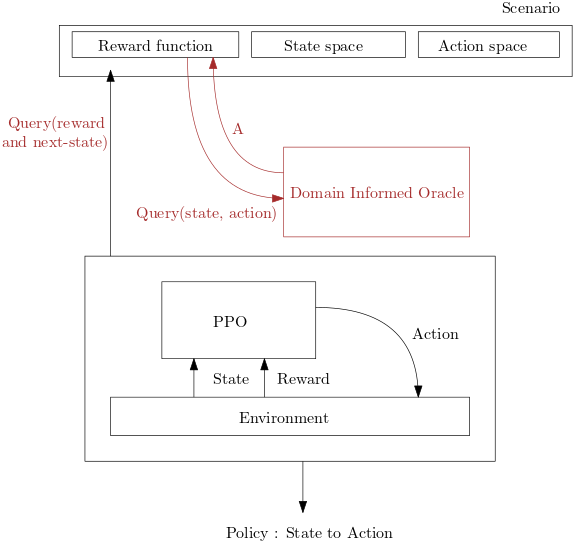
\includegraphics[width=1\linewidth]{figures/dio.png}
    \captionof{figure}{\dio{}+RL architecture}
    \label{fig:diorl}
  \end{minipage}
\end{figure}
\giselle{Are these figures still accurate? I thought you were no
longer using Q-learning.}

The diagram in Figure \ref{fig:basicrl} describes the basic routine of RL in more details. The environment defined by the scenario sends the current state 
to the Q-Learning algorithm. The agent chooses an action from the action space and sends it to the environment. This action affects the environment stepping it to some next state. 
The resulting state along its associated reward is computed from the reward function and step function formalized in the scenario. Thus, in the next iteration, the 
agent receives the reward from its previous action which it uses to improve its policy and continues with its training starting from the computed next state.  

\medskip 

The architecture in Figure \ref{fig:diorl} introduces \dio{} in the feedback loop. It is kept independent of the RL module. Precisely, when the scenario is query-ed for the reward and 
the resulting next state of a (state, action) pair, rather than computing the reward using the reward function, the latter is able to query \dio{}. The result of this query is $A$ which we keep 
obscure. The fundamental idea is that $A$ is used to inform the reward function when it is tasked with computing the reward. 
 

\subsection{\dio{} procedure}
\label{sec:modules}
In practice, we consider the following modules and their interactions as shown in \ref{fig:mods}.

\begin{enumerate}
  \item \textbf{World Rules} defining the rules governing the world. This is domain-dependent and implemented 
        in a logic programming file, i.e. we are able to define the next step via step semantics.
  \item \textbf{Knowledge Base} defining the ground facts which describe the world at a given time step. This module is 
        continuously updated to account for the dynamics of the
        state.
  \item \textbf{Labels} i.e., textual ``norms'' corresponding to an
  iteration of the state. In practice, they are all possible judgments on the resulting state, e.g. \textit{crash :- obs(X,Y), agent(X,Y)}, 
                  or \textit{maybecrash :- nextObs(X,Y), agent(X,Y)}. 
                    Those labels have probabilities associated with
                    them.
  \item \textbf{Translation Unit} defining the translation from state to ground facts and from labels to a numerical value, e.g. if the predicate crash is true with $P = 0.25$, then the reward shaped is $r + -0.25$. 
  \item \textbf{Reinforcement Learning} is our independent module that does not make assumption on the algorithm chosen for RL.
\end{enumerate}


\begin{figure}[H]
  \centering
  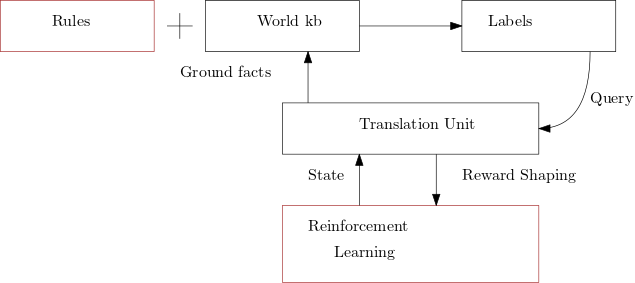
\includegraphics[scale=0.55]{figures/dynamics.png}
  \caption{Modules \& Interactions}
  \label{fig:mods}
\end{figure}

Figure \ref{fig:mods} describes the interactions of the different modules, basically taking a closure look to \dio{}. Precisely, 
given the rules and the world knowledge base at a given time $t$, we are able 
to produce the corresponding label, i.e. the query over a predicate. The predicate is fed 
into the Translation Unit (TU) that transforms the predicate to a numerical value that is given to the Reinforcement Learning 
as a reward shaping $r'$. This new reward can either \emph{overwrite} the previous reward, or \emph{fine-tune it}. In general, 
the way this reward affects the initial reward is a \textbf{design choice} that we leave for future investigations. 
Finally, as a result of the RL action, the next state is given 
to TU that translates it into Ground facts to update the world
knowledge, thus restarting the loop. Note that the inference on the query is done by a declarative tool that incorporates 
probabilities called \emph{Problog} that we introduce in \ref{sec:problog}.


\subsection{Problog Procedure} 
\label{sec:problog}
% High level overview of Problog
Problog is a logic programming language that aims to bridge between probabilistic 
logic programming and statistical relational learning \cite{fierens_van}. 
A problog program specifies a probability distribution over possible worlds. 
This probability distribution corresponds to the possible worlds whether a fact is taken 
or discarded given the probability associated with it. Precisely, they define a world 
is a subset of ground probabilistic facts where the probability of the subset is the product of 
the probabilities of the facts it contains.

\paragraph{Statistical Relational Learning (SRL)}
    Discipline of Artificial Intelligence that considers first order logic relations between 
    structures of a complex system and model it through probabilistic graphs such as Bayesian or 
    Markov networks.

\paragraph{Probabilistic Logic Programming (PLP)}
    Discipline of Programming Languages that augments traditional logic programming such as Prolog 
    with the power to infer over probabilistic facts to support the modeling of structured 
    probability distributions.


% Evidence and inference tasks in Problog
Furthermore, problog extends PLP with the power of considering evidences 
in the inference task. This is made possible without requiring the transformation 
the Bayesian networks on which to use SRL. Instead, problog considers the subset described above 
and assumes only worlds where the evidence held remains true. Those possible worlds and their associated 
probabilities are then added and divided by the choice with the higher probability. Problog makes this 
possible by a 3-steps conversion from a problog program to a weighted boolean formula.

% Conversion steps to weighted formula
First, problog grounds the program by only considering facts relevant to the query in question. 
The relevant ground rules are specifically converted to equivalent Boolean formulas. 
Precisely, inferences are converted into bi-directional implications and its corresponding premises 
are converted to a conjunction of disjunction of facts. 
Finally, problog asserts the evidence by adding it to the previous boolean formula 
as a conjunction and defines a weight function that assigns a weight to every literal. 
The weights are derived from the probability associated with the relevant literal, whether explicility 
given or implicility computed. 



%% Dynamic Obstacles in a GridWorld
\section{Dynamic Obstacles in a GridWorld} 
We first evaluate the performance of our dio/rl implementation compared to an implementation making only use of rl. 
\subsection{Scenario in Reinforcement Learning}
Our autonomous agent exists in an 8x8 grid world. Its goal is to reach the goal from his initial position (1,1).
Along the way, there exists dynamic obstacles which movements is unknown. The agent is punished if colliding with an obstacle and the episode, hereby ends. 
This environment offered by gym-gridworld \cite{gym_minigrid} is useful for testing our algorithm in a Dynamic Obstacle avoidance for a partially observable 
environment. Precisely, we define the state as follows. 
\begin{equation*}
  S_t = [x, y, d, G]
\end{equation*}
$(x,y)$ define the position of our agent while $d$ its direction. $G$ is the gridworld observed by the agent which includes walls, obstacles and free squares. 
The action space is, 
\begin{equation*}
  A_t = \{ right: 0, up: 1, down: 2, left: 3 \}
\end{equation*}
Finally, the reward is a function of the distance from the goal defined as, 
\begin{equation*}
  R_t = 1 - 0.9*(\dfrac{steps}{max\_steps})
\end{equation*}

\begin{multicols}{2}[\medskip]
    \begin{figure}[H]
      \centering
      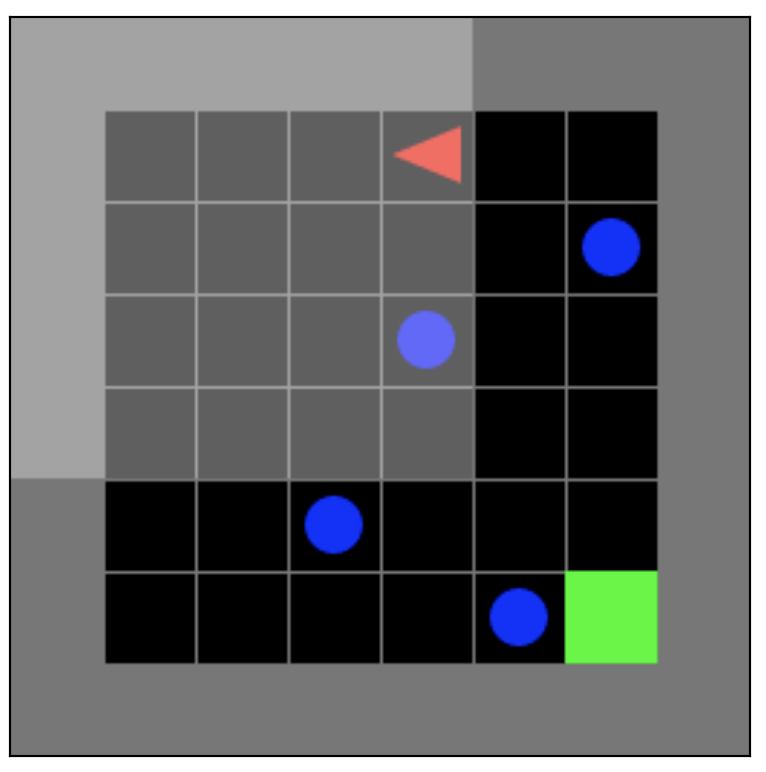
\includegraphics[scale=0.55]{figures/gridworldrl.png}
      \caption{Gridworld with Dynamic Obstacles}
      \label{fig:gridrl}
    \end{figure}
    \columnbreak
    The Reinforcement Learning experiments have been performed on 1M frames for a similar start configuration as shown in \ref{fig:gridrl}. The episode ends when the agent 
    reaches the goal OR collides with an obstacle. We want to encourage the shortest and safest path, thus, the punishment for crashing is $r = -1$. Our rewards are normalized as shown in
    the reward function. We define the range of rewards to be $(-1,1)$. 
\end{multicols}

\subsection{Domain Specific Rules}
\textcolor{red}{Fix the rules.}
The rules are defined as a ProbLog \cite{problog}: a probabilistic prolog that allows us to capture 
the stochasticity of the environment. Precisely, we want to consider the erratic movements of the obstacles, considering 
we do not have previous knowledge on the distribution of their given movement. We assume a uniform distribution and define the following. 
The rules of DIO take the following form: 

\begin{prooftree}
  \AxiomC{$p_1 \dots p_n$}
  \AxiomC{$\sum_{i=0}^{n}P(i) = 1$}
  \RightLabel{(action)}
  \BinaryInfC{$P_i :: \varphi(i)$}
\end{prooftree}
We define $\sum_{i=0}^{n}P(i) = 1$, and $\varphi(i)$ corresponds to the conjunction of grounds facts of the possible world with probability $P_i$.
The action is equivalent to our step semantics, thus, we enforce that a given action modifies the facts in some form. In practice, an action is the missing 
clause to generate the next predicate. In the gridworld example, we give the following. 

\begin{multicols}{2}
\begin{prooftree}
  \AxiomC{atPos(X + V*T, Y)}
  \RightLabel{(right)}
  \LeftLabel{(1)}
  \UnaryInfC{atPos(X,Y), speed(V), timestep(T)}
\end{prooftree}
\columnbreak 
\begin{prooftree}
  \AxiomC{0.25 :: obs(X + V*T, Y, V) \ldots}
  \LeftLabel{(2)}
  \RightLabel{(time)}
  \UnaryInfC{obs(X,Y,V), timestep(T)}
\end{prooftree}
\end{multicols}

(1) considers the movement of the agent while (2) considers the movement of the obstacles. Note that (2) considers 
a uniform distribution over the movement of the obstacle, since every obstacle has a uniform probability of moving up/down/left/right. 
We could do the same for (1) by consider the probability of an action failing. In our case, we assume the movement is deterministic and no failure over the movement 
of the agent happens.


\subsection{World Knowledge}
Our world knowledge base covers the agent, the obstacles and the timestep. We consider two cases: 
\textit{constant} ground facts vs. \textit{dynamic} ground facts. The latter represents positions which are dynamically 
generated at every timestep while the former considers only the facts that remain true in every world, thus include the timestep, since we always
move by 1-unit, and the speed, since the agent and the obtacles are defined to only move by 1-box every time. Given that our knowledge base $Kb$ is defined by, 
\[
    C = \{speed(1), timestep(1) \}     
    \qquad
    D = \{atPos(X, Y), obs(X,Y,1)\}
    \qquad
    Kb = C \cup D
\]

\subsection{From Norms to Labels}
In the following, we define \textbf{\glsplural{norms}} as textual sentences to describe the intended goal behavior. 
Thus, in the gridworld example, we consider three possibles norms, (1) \textit{crash} when the agent and the obstacle overlap, (2) \textit{maybecrash} 
when the agent and the obstacle are one square from each other and finally (3) \textit{safe} when there is ample distance between the agent the obstacle 
in this case, two square distances. Those norms are identified as 'labels', i.e. predicates defined as follows. 

\[
    \infer{1 :: crash}{1 :: atPos(X,Y) & 1 :: obs(X,Y,\_)} 
    \qquad
    \infer{P_1 \times P_2 :: maybecrash}{P_1::atPos(X,Y), P_2::obs(X,Y,\_)
      & \ldots}
\] 
\[
    \infer{P_1 \times P_2 :: safe}{
      P_1::atPos(X_1,Y_1), P_2::obs(X_2,Y_2,\_),X_1 \neq X_2, Y_1 \neq Y_2
      & \ldots
    }
\]
\[
  \infer{1.0/(L+T) :: close}{
    nextPos(X,Y), goal(I,J), time(T), L = abs(I-X) + abs(Y-J)
  }
\]

 \paragraph{Nondeterminism} 
 If we look at crash and maybecrash predicates, we notice that the two hold for the 
 same premises. This is what we define as non-determinism, where any of the two can be chosen. 
 The choice was made considering that a crash would imply a 'maybecrash', thus trivially true. 

\subsection{Translation Unit}
The translation unit is the bridge between Dio and RL. Precisely, it handles both feeding 
the world facts to Dio and translates the feedback given to a numerical value, through 
a given function. First, the Dio/RL loop is given in Algorithm 1. 

  \begin{algorithm}[H]
    \caption{Dio/RL Loop}
    \begin{algorithmic}[1]
    
    \Procedure{Step}{$S_t, a$}       \Comment{(State, action) Pair}
        \State Check for invalid actions
        \State Check for obstacles 
        \State Update Obstacles positions
        \State Update Agent's position
        \State \textbf{UpdateWorld}(position, direction, obstacles) \Comment{KB update in DIO}
        \State $obs, reward$ = Step'$(S_t, ac)$ \Comment{Call to Initial Env}
        \State $reward'$ = \textbf{getFeedback()} \Comment{Query DIO}
        \If{$reward' != -1$} 
            \State $reward$ += reward'
        \EndIf
        \State return (obs,reward)
    \EndProcedure
    
    \end{algorithmic}
    \end{algorithm}

When it comes to reward shaping, we focus on the 'getFeedback' function. First, the translation units gets 
the labels, i.e. the probabilities of the evaluated predicates and constructs a function that associates 
every predicate to its corresponding numerical value. Finally, the reward is equivalent to weighted probabilities 
as shown in Algorithm 2.

\begin{algorithm}[H]
  \caption{Reward Shaping from RL to DIO/TU}
  \begin{algorithmic}[1]
      
      \Procedure{getFeedback}{} 
      \State labels $\gets$ \textbf{getLabels()} \Comment{Evaluated predicates w/ Corresponding Probabilities}
      \State $P \gets \{$crash, maybecrash, safe$\}$  \Comment{Set of possible worlds}
      \State $F \gets \{-1,-0.5,1\}$ \Comment{Numerical value associated with world}
      \State $i \gets 1$
      \State $r \gets 0$
      \While{$i \leq$ length(labels)} 
         \State $r \gets r +$ labels[P[i]]*F[i] \Comment{Equivalent to weighted probabilities}
         \State $i \gets i+1$


      \EndWhile
      
      \EndProcedure
      
      \end{algorithmic}
      \end{algorithm}

    \subsection{Preliminary Results}
    Our testing was done on a Dynamic Obstacles grid world using proximal policy optimization over 80k frames. 
    We pick up the frames per second to evaluate the speed of learning, the mean number of frames per episode 
    to evaluate the optimality of the solution and finally, the mean returns per episode to evaluate convergence relative 
    to the number of frames. The code is available on github \cite{dio} with steps on how to replicate our model.

    \begin{figure}[H]
      \centering
      \begin{minipage}{.4\textwidth}
        \centering
        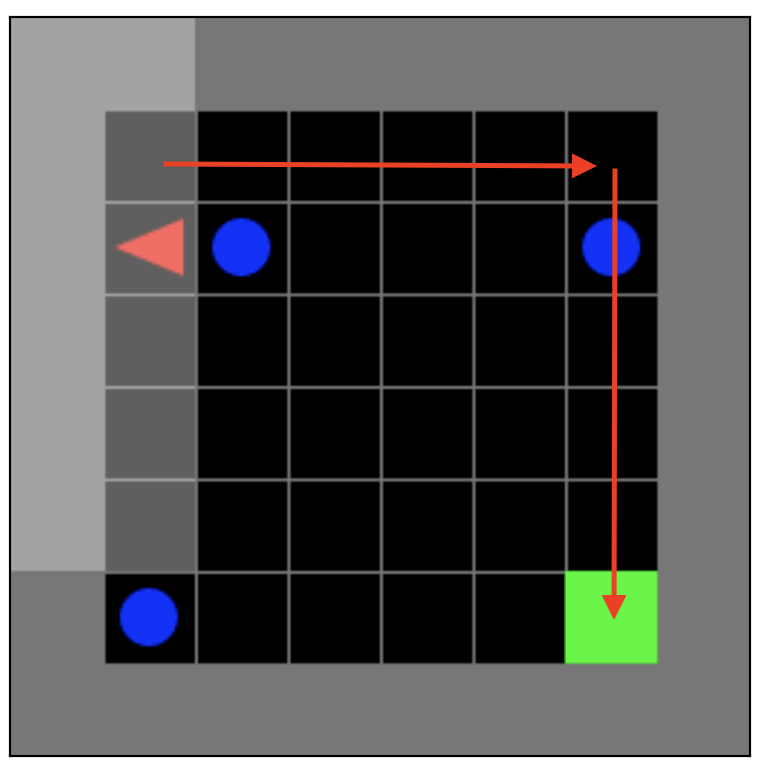
\includegraphics[width=1\linewidth]{figures/diopolicy.png}
        \captionof{figure}{\Gls{policy} learned with Dio}
        \label{fig:policydio}
      \end{minipage}%
      \begin{minipage}{.4\textwidth}
        \centering
        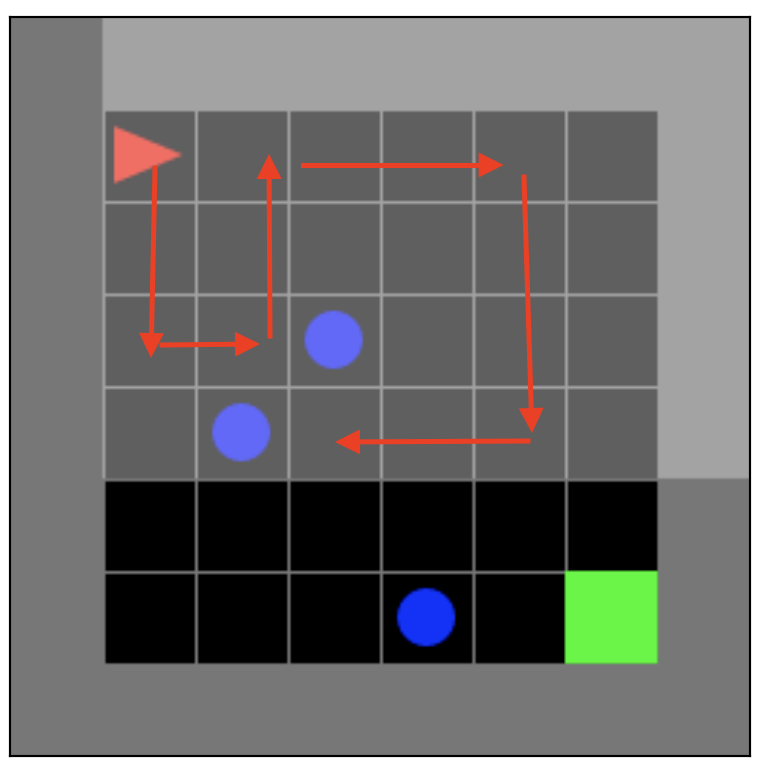
\includegraphics[width=1\linewidth]{figures/rlpolicy.png}
        \captionof{figure}{Policy learned without Dio}
        \label{fig:policyrl}
      \end{minipage}
    \end{figure}

    We first visualized the learned policy in the two implementations. Althrough both learned 
    how to not crash into the Dynamic Obstacles, the implementation with Dio was better at minimizing the number of steps 
    but also learned to reach the goal. 


    \begin{figure}[H]
      \centering
      \begin{minipage}{.5\textwidth}
        \centering
        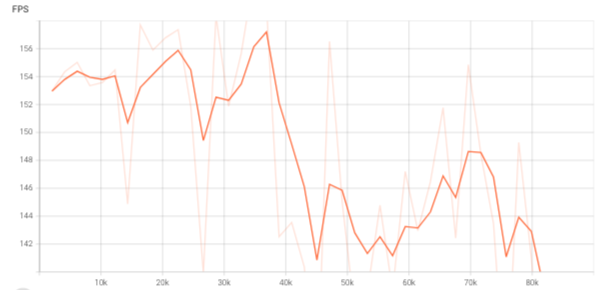
\includegraphics[width=1\linewidth]{figures/diofps.png}
        \captionof{figure}{Frames per Second with Dio}
        \label{fig:fpsdio}
      \end{minipage}%
      \begin{minipage}{.5\textwidth}
        \centering
        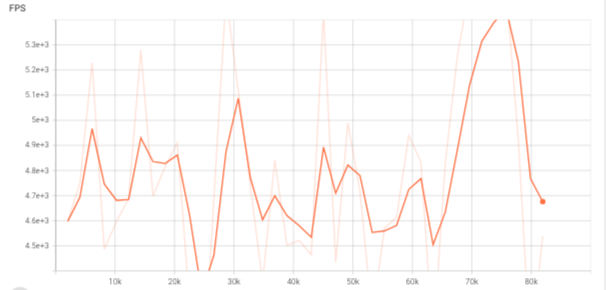
\includegraphics[width=1\linewidth]{figures/rlfps.png}
        \captionof{figure}{Frames per Second without Dio}
        \label{fig:fpsrl}
      \end{minipage}
    \end{figure}

    First, as expected, the implementation using Dio is much slower only able to run 
    an average of 150 episodes per second. As a result, for 80k episodes, the implementation with Dio 
    took 9 minutes to train versus 16 seconds for the implementation without. However, this loss in time shows as in \ref{fig:framesdio} 
    a gain in optimality. When visualizing the learned policy of Dio, we found that our agent succeeds in 90\% 
    of the time to reach the goal without colliding taking an average of $50 \pm 21$. Consider that 
    the optimal number of steps without obstacles is 13, while the policy learned without Dio did not reach a suitable solution and fails to 
    not collide 17\% of the time. When it does reach a solution, it takes an average of $231 \pm 59$ to reach the goal. 


    \begin{figure}[H]
      \centering
      \begin{minipage}{.5\textwidth}
        \centering
        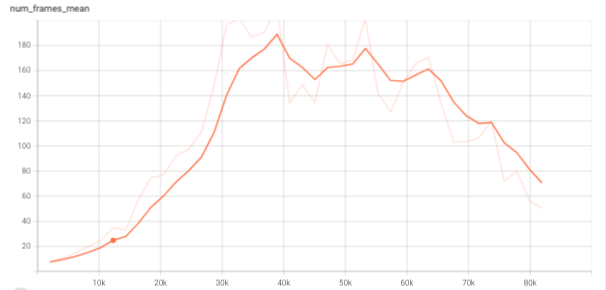
\includegraphics[width=1\linewidth]{figures/dioframesmean.png}
        \captionof{figure}{Mean of \glspl{frame} per episode with Dio}
        \label{fig:framesdio}
      \end{minipage}%
      \begin{minipage}{.5\textwidth}
        \centering
        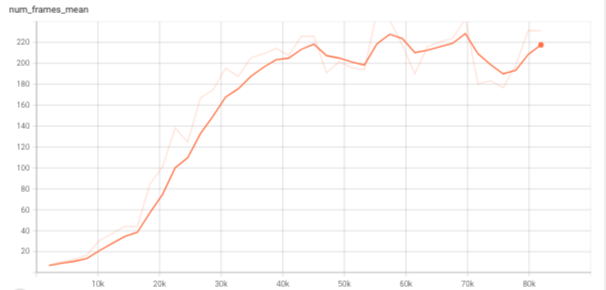
\includegraphics[width=1\linewidth]{figures/rlframesmean.png}
        \captionof{figure}{Mean of frames per episode without Dio}
        \label{fig:framesrl}
      \end{minipage}
    \end{figure}

    The dip in the mean frames in \ref{fig:framesdio} show that the agent did not only learn 
    how to only collide but also is learning how to reach the goal in the shortest amount of time. 
    Since \ref{fig:returndio} is still increasing, we can also tell that the values did not converge yet and 
    the agent can learn even a better optimization while \ref{fig:returnrl} shows that the values converge towards
    a suboptimal policy.

    \begin{figure}[H]
      \centering
      \begin{minipage}{.5\textwidth}
        \centering
        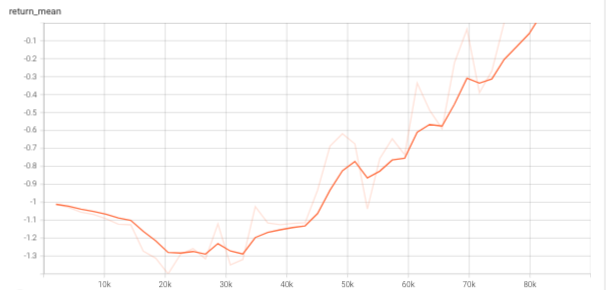
\includegraphics[width=1\linewidth]{figures/dioreturn.png}
        \captionof{figure}{Mean of \glspl{return} per episode with Dio}
        \label{fig:returndio}
      \end{minipage}%
      \begin{minipage}{.5\textwidth}
        \centering
        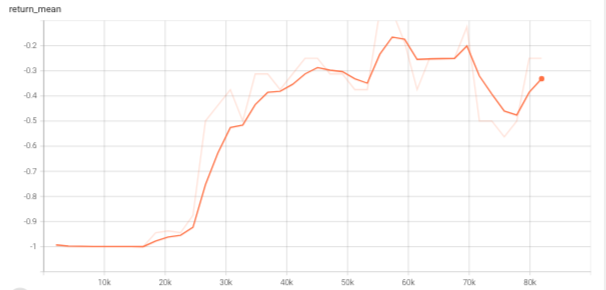
\includegraphics[width=1\linewidth]{figures/rlreturn.png}
        \captionof{figure}{Mean of returns per episode without Dio}
        \label{fig:returnrl}
      \end{minipage}
    \end{figure}

    In \ref{fig:returndio} and \ref{fig:returnrl}, it is evident that the policy learned by Dio 
    is more optimal. Similarly, when evaluating our policies on the same reward scheme, 
    the implementation with dio averages a 0.64 while without dio averages a -0.18 return.

    Overall, the results show that an implementation that makes use of dio is beneficial even in a stochastic environment. 
    As we lose in speed, we gain in optimality of the solution. 
    Given those preliminary results, we want to (1) optimize our implementation 
    and (2) test our implementation in a more complex scenario that requires a more complex understanding of the world 
    from dio's side. (1) is discussed in \ref{optimality} and (2) is discussed in \ref{traffic}. 



%% Traffic Simulation using Carla
\section{Traffic Simulation} 
\label{traffic}

Given the definition of our DIO architecture, the performance as shown in Figure \ref{fig:overview} will be judged on a Traffic Simulation. 
Precisely, we make use of the OpenSource code of Carla \cite{Dosovitskiy17} to put our implementation in practice. 
\subsection{Scenario in Reinforcement Learning}
Our autonomous agent is one vehicle on the road. The road is populated with other vehicles, walkers and traffic signs and lights. 
The goal of the agent is to get from point $A$ to point $B$ on the map in the fastest time possible. Carla defines \emph{sensors} to collect 
data from the world. From the sensors, we collect \textbf{collision detector}, \textbf{obstacle detector}, \textbf{IMU} (which defines the internal state of the vehicle that includes acceleration)
and finally \textbf{position} data to incorporate into our state representation. Thus, 
\begin{equation*}
  S_t = [t, p, c, o, a]
\end{equation*} 
In other words, the state at time $t$ is defined by $t$ the time, $p$ the position and $a$ the acceleration. $c$ and $o$ are both flags (-1/1) that indicate 
respectively whether there is a collision or an obstacle detected. (-1) is equivalent to detected while (1) is equivalent to non-detected. Furthermore, 
\begin{equation*}
  A_t = ](a_t)-min, (a_t)+max[
\end{equation*}
Precisely, our action space at time $t$ is a range delimited by the minimum acceleration possible and the maximum acceleration possible. Finally, 
\begin{equation*}
  R_t(s_t) = c * (d(i, p)/t) + (o * a)
\end{equation*}
We define $d$ a function that takes in the initial position $i$ and the current position $p$ and computes the distance travelled. 
By putting everything together, we can see that the reward is maximized when the agent travels the longest distance in a shortest 
amount of time (without colliding at high speed) while making sure that when an obstacle is detected, acceleration is kept low. 

\subsection{Domain Specific Rules in DIO}

Note that DIO is a logic programming module that we design in Prolog and 
carry to Python via PySwip \cite{tekol2020}.
The first step of DIO is to consider the translation. 
\[
  \infer[T_1]{[t, p, -1, 1, a]}{\text{Time}(t) \wedge \text{Pos}(p) 
                                \wedge \text{Acc}(a) \wedge
                              \text{Collision}}
   \qquad
   \infer[T_2]{[t, p, -1, -1, a]}{\text{Time}(t) \wedge \text{Pos}(p) 
                                  \wedge \text{Acc}(a) \wedge
                                  \text{Collision} \wedge \text{Obstacle}}
\]

\[
  \infer[T_3]{[t, p, 1, 1, a]}{\text{Time}(t) \wedge \text{Pos}(p) 
                                \wedge \text{Acc}(a)
                            }
   \qquad
   \infer[T_4]{[t, p, 1, -1, a]}{\text{Time}(t) \wedge \text{Pos}(p) 
                                  \wedge \text{Acc}(a) \wedge \text{Obstacle}}
\]

The domain specific rules will follow the same idea, taking in the ground facts and the action, 
and infering the next set of ground facts. Thus, DIO searchs for configurations of ground facts given the step semantics, 
to return the set of labels. The main challenge is pruning the search space as we want to 
guarantee time efficiency. While we hypothesize that the RL would learn faster by incorporating 
domain knowledge, we are expecting iterations to take longer as the feedback loop incorporates DIO's computation. This part is an ongoing work. 


%% Input for related work
%% Remember to mention more on reward shaping and domain informed approaches to ML
\section{Related Work}

As discussed previously in Section \ref{symrl}, neurosymbolic AI trends show promising results in improving ML algorithms, whether that is from 
an interpretability aspect or an optimization one. More recent works take this trend and incorporate symbolic reasoning and 
domain knowledge in reinforcement learning settings \cite{Driessens2010,Romero2020,achiam2017,marek2010}. \cite{marek2010,Romero2020} use the general idea of \textit{reward shaping} and \textit{epsilon adaptation} respectively 
to incorporate procedural knowledge into a RL algorithm. Both introduce this combination as a successful strategy to guide the exploration and exploitation tradeoff in RL. They both show promising results. While 
\cite{marek2010} focuses on providing formal specifications for reward shaping, it lacks practical 
consequences to the implementation of most RL to make use of its formal methods conclusions. On the other hand, \cite{Romero2020} proposes a method to adapt $\epsilon$ based on domain knowledge, the method is specifically applied to "Welding Sequence Optimization".  
To do so, the RL algorithm is modified in itself, similarly to what was done in \cite{Driessens2010}. Precisely, in \cite{Driessens2010}, the RL algorithm itself is 
modified to deal with states that are model-based as opposed to vectors. They defined their method as Relational RL. 
Furthermore, they conclude that by using more expressive representation language for the RL scenario, their method can be potentially offer a solution to the problem of meta-learning. 
While \cite{Romero2020,Driessens2010} both present promising rewards, they lack the modularity necessary for scaling the proposed methods to further RL implementations. Those by taking their results into consideration, 
we are hopeful that symbolic reasoning and RL integration could provide a solution for reward shaping, meta-learning and the exploration-exploitation dilemma. 


\section{Conclusions}

In conclusion, as RL faces the issues of reward shaping, meta-learning and the exploration-exploitation dilemma, domain knowledge show promising results in 
improving reinforcement learning methods. The main challenge is to make such an integration seamless, and independent of the AI implementation. 
As we start incorporating our modules into one architecture to test on our Traffic Simulator in Section \ref{traffic}, we will be able to show preliminary 
results. Similarly, we look further into the specifications of DIO to ensure that it informs the scenario in a meaningful way as discussed in Section \ref{scspecs}. 

\newpage

\bibliographystyle{unsrt}
\bibliography{biblio.bib}

% Commenting this in/out to include/exclude the appendix
\newpage

\appendix
\section{Appendix}

In the following, we describe our previous work that was done towards considering safe reinforcement learning. 
Precisely, we were motivated by the lack of safety guarantees and the use of symbolic reasoning towards incorporating 
safety properties from a verified safe controller (SC) i.e. a declarative language module to compute safe and unsafe states. 
Those safety states are computed during training, thus ensuring that no unsafe states are explored 
by the RL. The general idea was to allow training in the real-world, thus taking away the need for simulation. Our proposed RL+SC architecture is shown in Figure \ref{fig:rlsc}.


\begin{figure}[H]
  \centering
  
\includegraphics[scale=0.5]{rlsc.png}
  \caption{Overview of the proposed solution}
  \label{fig:rlsc}
\end{figure}

\begin{enumerate}
  \item The environment sends the observation to the SC. 
  \item The SC computes the state from the observation, thus keeping only 
        ground facts that uphold the \emph{Markov Property} (see Definition 9.1). 
  \item The SC also computes the set of possible actions $A$ that ensure that no unsafe states is 
        reached. This is done by searching for possible configurations that follow a (state, action) pair over 
        all possible actions from the action spaces. 
  \item The state and set of possible actions is sent to the RL algorithm, thus only allowing 
        the agent to choose from the set actions. 
  \item Next steps follow from the RL basic routine from Figure \ref{fig:rl}
\end{enumerate}

The implementation can be found in the thesis corresponding github under the rl-implementation folder\footnote{https://github.com/natvern/Thesis}.
For our case study, we chose the vehicle platooning problem. The setting is as follows; two vehicles, one leader and one follower. Their goal is to 
minimize the gap between them while ensuring that they do not crash. 

\medskip

We then present our preliminary results before arguing for the issues with our approach. 

\begin{figure}[H]
  \centering
  \begin{minipage}{.5\textwidth}
    \centering
    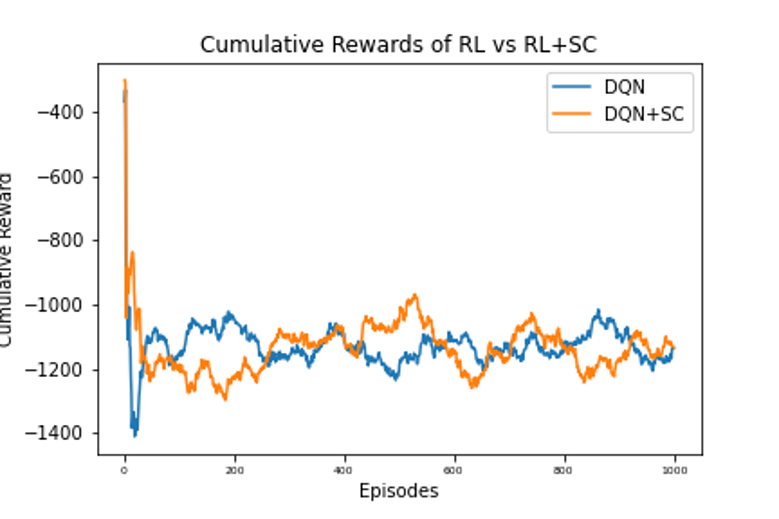
\includegraphics[width=1\linewidth]{appendixopt.png}
    \captionof{figure}{Cumulative Rewards of RL vs. RL+SC}
    \label{fig:optsc}
  \end{minipage}%
  \begin{minipage}{.5\textwidth}
    \centering
    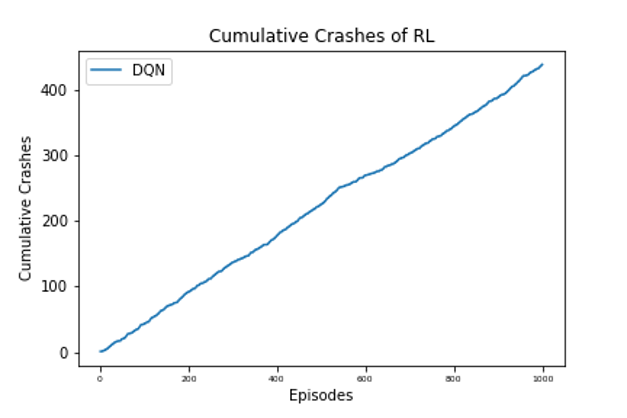
\includegraphics[width=1\linewidth]{appendixcrash.png}
    \captionof{figure}{Cumulative Crashes of RL during Training}
    \label{fig:crashsc}
  \end{minipage}
\end{figure}
  
The graph in Figure \ref{fig:optsc} shows the cumulative rewards of the basic RL implementation without
the safe controller (blue line) vs. the RL+SC implementation (orange line). As evident in the cumulative rewards, all are negative. This is because of our reward function choice 
that only punishes for distances not equal to the desired gap. Thus, learning is not optimal. We can however see that the cumulative rewards of both implementation does not change by a significant 
amount. The graph in Figure \ref{fig:crashsc} shows 
the number of crashes of the basic RL during training. We can easily deduce from the linear graph that the RL without the SC never learns not to crash.


\begin{definition}[Markov Property]
  The next state only depends on the value of the current state. In other words, only the present can affect the future. 
  In terms of our state vector, this means that given $S_t$, I only need the features in $S_t$ to predict $S_{t+1}$.
\end{definition}

\subsection{Issues with the safe RL approach}
\begin{itemize}
  \item The simplicity of our problem setting does not showcase the need for a SC as we only consider two vehicles on an x-axis. 
  \item Though ensuring safety guarantees during training theoretically takes away the need for a simulation, in practice, the uncertainties 
        of the real world cannot be all predicted. This results in a handful of safety properties that might be guaranteed, not enough to allow sensitive cyber-physical systems 
        to be trained using RL in the real world. 
  \item If an oracle existed that was able to predict all uncertainties of the real world, this oracle could then be used to solve the optimization problem 
        deterministically without the need for RL. 
  \item Depending on the SC implementation, safety guarantees can be too strict thus completely destroying optimality. Consider a SC that only allows a car not to move. 
        Though it guarantees that no crashes happen, it is also too strict, thus going against the goal of the agent. 
  
\end{itemize}




\end{document}
